% ============================================================
%  Final Project Report
%  Deepfake Image Detection Using Frequency-Domain Analysis
%  and Explainable AI
%
%  Bahcesehir University — AI Engineering — 2026
%  Author: Kenan Eliyan
%
%  Compile with:
%    pdflatex report.tex
%    bibtex   report
%    pdflatex report.tex
%    pdflatex report.tex
% ============================================================

\documentclass[12pt, a4paper]{article}

% ── Geometry ─────────────────────────────────────────────────────────────────
\usepackage[
  top=2.5cm, bottom=2.5cm,
  left=3.0cm, right=2.5cm
]{geometry}

% ── Language & encoding ──────────────────────────────────────────────────────
\usepackage[T1]{fontenc}
\usepackage[utf8]{inputenc}
\usepackage{lmodern}

% ── Mathematics ──────────────────────────────────────────────────────────────
\usepackage{amsmath, amssymb}

% ── Graphics & figures ───────────────────────────────────────────────────────
\usepackage{graphicx}
\usepackage{subcaption}
\usepackage{float}

% ── Tables ───────────────────────────────────────────────────────────────────
\usepackage{booktabs}
\usepackage{array}
\usepackage{multirow}
\usepackage{tabularx}

% ── Hyperlinks ───────────────────────────────────────────────────────────────
\usepackage[
  colorlinks=true,
  linkcolor=blue!70!black,
  citecolor=blue!70!black,
  urlcolor=blue!70!black
]{hyperref}

% ── Listings (code) ──────────────────────────────────────────────────────────
\usepackage{listings}
\usepackage{xcolor}
\lstset{
  basicstyle=\ttfamily\small,
  breaklines=true,
  frame=single,
  backgroundcolor=\color{gray!8},
  commentstyle=\color{green!50!black},
  keywordstyle=\color{blue!70!black}\bfseries,
  stringstyle=\color{orange!80!black},
  numbers=left,
  numberstyle=\tiny\color{gray},
  numbersep=6pt,
}

% ── Spacing & typography ─────────────────────────────────────────────────────
\usepackage{setspace}
\onehalfspacing
\usepackage{microtype}
\usepackage{parskip}
\setlength{\parskip}{6pt}

% ── Headers & footers ────────────────────────────────────────────────────────
\usepackage{fancyhdr}
\pagestyle{fancy}
\fancyhf{}
\lhead{\small Deepfake Detection via Frequency Analysis}
\rhead{\small Kenan Eliyan — BAU AI Engineering 2026}
\cfoot{\thepage}
\renewcommand{\headrulewidth}{0.4pt}

% ── Section formatting ───────────────────────────────────────────────────────
\usepackage{titlesec}
\titleformat{\section}{\large\bfseries}{\thesection.}{0.5em}{}
\titleformat{\subsection}{\normalsize\bfseries}{\thesubsection.}{0.5em}{}
\titleformat{\subsubsection}{\normalsize\itshape}{\thesubsubsection.}{0.5em}{}

% ── Miscellaneous ─────────────────────────────────────────────────────────────
\usepackage{enumitem}
\usepackage{caption}
\captionsetup{font=small, labelfont=bf, skip=4pt}

% ── Bibliography ─────────────────────────────────────────────────────────────
% Uses plain BibTeX (natbib-free) — compile: pdflatex → bibtex → pdflatex ×2
\bibliographystyle{ieeetr}

% ─────────────────────────────────────────────────────────────────────────────
%  Title block
% ─────────────────────────────────────────────────────────────────────────────
\title{%
  \vspace{-1cm}
  \Large\textbf{Deepfake Image Detection Using\\
  Frequency-Domain Analysis and Explainable AI}\\[0.8em]
  \normalsize Final Project Report — AI Engineering\\
  Bahcesehir University, Istanbul
}
\author{%
  \textbf{Kenan Eliyan}\\[0.3em]
  \normalsize AI Engineering, Faculty of Engineering and Natural Sciences\\
  Bahcesehir University\\
  \texttt{kenan.eliyan@std.bau.edu.tr}
}
\date{May 2026}

% ─────────────────────────────────────────────────────────────────────────────
\begin{document}
% ─────────────────────────────────────────────────────────────────────────────

\maketitle
\thispagestyle{empty}

% ── Abstract ─────────────────────────────────────────────────────────────────
\begin{abstract}
\noindent
The rise of high-fidelity face-synthesis methods, particularly Generative
Adversarial Networks (GANs), has made deepfake imagery increasingly difficult to
detect by visual inspection alone.  This project investigates whether combining
spatial (RGB) and spectral (FFT) cues in a unified deep neural network
outperforms either modality in isolation for binary real/fake face
classification.  Three detection strategies are implemented and benchmarked
under identical conditions: an RGB-only ResNet18 model fine-tuned from ImageNet
weights, an FFT-only ResNet18 model trained from scratch on log-magnitude
frequency spectra, and a Hybrid dual-branch model that fuses features from both
domains through late concatenation.  All experiments are conducted on a balanced
30,000-image subset of the publicly available ``140K Real and Fake Faces''
Kaggle dataset, which contains real photographs (FFHQ/Flickr) alongside
StyleGAN2-generated counterparts.  Evaluation on a held-out test split of 4,500
images shows that the Hybrid model achieves 99.5\% accuracy and a ROC-AUC of
0.9998, matching or surpassing the strong RGB baseline (99.0\%, AUC
0.9975), while the FFT-only model reaches only 61.0\% accuracy (AUC 0.6412) —
barely above random chance.  Gradient-weighted Class Activation Mapping
(Grad-CAM) is applied to both the RGB and Hybrid models to produce visual
explanations of which image regions drive each prediction, revealing that the
RGB branch consistently focuses on high-level facial structure.  The results
confirm that frequency artifacts alone are insufficient for reliable
StyleGAN2-face detection, yet their inclusion in a dual-branch architecture
eliminates all false negatives, achieving perfect recall.  Code, metrics, and
all generated figures are publicly available on GitHub.

\smallskip
\noindent\textbf{Keywords:} deepfake detection, GAN artifacts, frequency
analysis, FFT, ResNet18, Grad-CAM, explainable AI, image forensics
\end{abstract}

\newpage
\tableofcontents
\newpage

% ─────────────────────────────────────────────────────────────────────────────
\section{Introduction}
\label{sec:intro}
% ─────────────────────────────────────────────────────────────────────────────

Deepfake technology, which uses deep generative models to synthesise or
manipulate facial images and videos, poses serious challenges for digital
trust, media authenticity, and personal privacy~\cite{goodfellow2014gan}.
Early GAN-based deepfakes were easily identifiable by trained observers, but
the introduction of progressive and style-based architectures — most notably
StyleGAN and StyleGAN2~\cite{karras2020stylegan2} — has produced synthetic
faces that are perceptually indistinguishable from real photographs to the
human eye.

Two broad families of detection approaches have emerged in the literature.
\emph{Spatial-domain} methods apply convolutional neural networks (CNNs)
directly to pixel-space images, exploiting subtle texture or structural
inconsistencies left by the synthesis
process~\cite{rossler2019faceforensics}.  \emph{Frequency-domain} methods
instead analyse the Fourier or DCT spectrum of the image, motivated by the
observation that transposed-convolution upsampling layers introduce periodic
spectral artifacts that are absent from photographs of real
scenes~\cite{frank2020frequency, dzanic2020fourier, durall2019unmasking}.

This project sits at the intersection of both approaches.  The central
hypothesis is:
\begin{quote}
\emph{A dual-branch model that jointly processes spatial (RGB) and spectral
(FFT) features outperforms either modality alone on StyleGAN2 face detection.}
\end{quote}

Three experiments are conducted to test this hypothesis:
\begin{enumerate}[leftmargin=1.8em]
  \item \textbf{RGB baseline} — a ResNet18~\cite{he2016resnet} fine-tuned from
    ImageNet weights on raw $224 \times 224$ face images.
  \item \textbf{FFT model} — an identical ResNet18 trained from scratch on
    per-channel log-magnitude FFT spectra.
  \item \textbf{Hybrid model} — a dual-branch architecture that fuses 512-d
    features from both branches through late concatenation, followed by a
    two-layer classification head.
\end{enumerate}

All models are augmented with Grad-CAM~\cite{selvaraju2017gradcam}
visualisations to provide post-hoc spatial explanations of their predictions.

The remainder of this report is organised as follows.
Section~\ref{sec:related} reviews related work.
Section~\ref{sec:dataset} describes the dataset and preparation procedure.
Section~\ref{sec:method} details the preprocessing pipeline, model
architectures, and training configuration.
Section~\ref{sec:experiments} presents experimental results and analysis.
Section~\ref{sec:gradcam} discusses the Grad-CAM visualisations.
Section~\ref{sec:conclusion} concludes with future research directions.

% ─────────────────────────────────────────────────────────────────────────────
\section{Related Work}
\label{sec:related}
% ─────────────────────────────────────────────────────────────────────────────

\subsection{Spatial-domain Detection}

The FaceForensics++ benchmark~\cite{rossler2019faceforensics} provided an
early, rigorous evaluation platform for deepfake detectors.  A fine-tuned
XceptionNet on compressed video frames achieved compelling results on five
manipulation types, establishing spatial CNNs as a strong baseline.  The
success of ImageNet-pretrained networks on deepfake detection tasks has since
been replicated across many architectures, suggesting that low-level texture
statistics learned from natural images transfer well to identifying synthetic
artefacts.

\subsection{Frequency-domain Analysis}

Durall et al.~\cite{durall2019unmasking} were among the first to demonstrate
systematically that GAN-generated images exhibit characteristic frequency
fingerprints: an elevated high-frequency energy distribution that differs from
the natural image prior.  They showed that even a simple classifier operating
on the 1D azimuthal power spectrum can separate real from GAN-generated faces
with reasonable accuracy.

Frank et al.~\cite{frank2020frequency} built on this by applying 2D DCT
spectra as input features to CNNs, reporting detection rates above 90\% for
several GAN architectures.  They also showed that frequency-based detectors
degrade when images are JPEG-compressed — a finding that underscores the
practical limitations of spectral approaches.

Dzanic et al.~\cite{dzanic2020fourier} provided a theoretical explanation
for the spectral discrepancies: transposed-convolution layers used for
upsampling in most GAN decoders create a periodic ``checkerboard'' pattern in
the frequency domain due to uneven overlap of the convolutional kernel.

\subsection{Hybrid and Multi-modal Approaches}

Several works have explored combining spatial and frequency cues.  F3Net
(Qian et al., 2020) uses frequency-aware decomposition and local texture
analysis in a multi-stream network, achieving state-of-the-art results on
FaceForensics++.  The present project differs in scope and simplicity:
instead of a specialised frequency decomposition, raw 2D FFT spectra are fed
directly into an unmodified ResNet18, making the approach straightforward to
replicate and extend.

\subsection{Explainability in Deepfake Detection}

Class Activation Mapping (CAM)~\cite{zhou2016cam} and its gradient-based
generalisation Grad-CAM~\cite{selvaraju2017gradcam} have been adopted as
standard tools for interpreting CNN decisions.  In deepfake detection,
heatmaps have revealed that well-performing models often attend to the eye
and mouth regions — areas where GAN synthesis tends to introduce the most
visible inconsistencies.  This report applies Grad-CAM to both the RGB and
Hybrid models to verify that their spatial attention is semantically
meaningful.

% ─────────────────────────────────────────────────────────────────────────────
\section{Dataset}
\label{sec:dataset}
% ─────────────────────────────────────────────────────────────────────────────

\subsection{Source Data}

The ``140K Real and Fake Faces'' dataset~\cite{dataset140k} from Kaggle
provides 70,000 real face photographs sourced from the
FFHQ~\cite{karras2020stylegan2} and Flickr collections, paired with 70,000
synthetic faces generated by StyleGAN2.  All images are pre-aligned, cropped
to $256 \times 256$ pixels, and contain a single frontal face.  The
balanced real/fake composition ensures that a trivial majority-class
classifier would achieve exactly 50\% accuracy — any improvement over this
baseline is attributable to genuine learned features.

\subsection{Subset Selection and Splitting}

Because the full 140,000-image dataset would require substantial storage and
training time, a balanced 30,000-image subset was selected using a
reproducible procedure (random seed = 42).  The subset is split into training,
validation, and test partitions at a 70\,/\,15\,/\,15 ratio, maintaining
class balance across splits.  Table~\ref{tab:split} summarises the resulting
partition sizes.

\begin{table}[H]
\centering
\caption{Dataset partition sizes used in all three experiments.}
\label{tab:split}
\begin{tabular}{lrrr}
\toprule
\textbf{Split} & \textbf{Real} & \textbf{Fake} & \textbf{Total} \\
\midrule
Train & 10,500 & 10,500 & 21,000 \\
Validation & 2,250 & 2,250 & 4,500 \\
Test & 2,250 & 2,250 & 4,500 \\
\midrule
\textbf{Total} & \textbf{15,000} & \textbf{15,000} & \textbf{30,000} \\
\bottomrule
\end{tabular}
\end{table}

The preparation script (\texttt{src/prepare\_data.py}) implements an additive
strategy: if a previous run has already populated some destination folders,
subsequent runs only add the \emph{missing} images to reach the per-folder
targets.  This prevents accidental data leakage that would arise from
naively re-splitting an already-populated directory.

\subsection{Data Augmentation}

During training, the following transforms are applied to each image
on-the-fly to improve generalisation:
\begin{itemize}[leftmargin=1.8em]
  \item Resize to $224 \times 224$ pixels (bilinear interpolation)
  \item Random horizontal flip with probability 0.5
  \item Colour jitter: brightness $\pm 0.1$, contrast $\pm 0.1$,
    saturation $\pm 0.05$
  \item Normalisation to ImageNet statistics
    ($\mu = (0.485, 0.456, 0.406)$, $\sigma = (0.229, 0.224, 0.225)$)
\end{itemize}

Validation and test images receive only the resize and normalisation steps;
no stochastic augmentation is applied at inference time.

% ─────────────────────────────────────────────────────────────────────────────
\section{Methodology}
\label{sec:method}
% ─────────────────────────────────────────────────────────────────────────────

\subsection{FFT Preprocessing Pipeline}
\label{sec:fftpre}

The core novelty of the FFT and Hybrid branches lies in the conversion of a
normalised RGB image into a frequency-domain representation suitable for
ResNet18 input.  The pipeline is applied per-channel and proceeds as follows:

\begin{enumerate}[leftmargin=1.8em]
  \item \textbf{Denormalise.}  ImageNet mean and standard deviation are
    reversed to recover pixel values in $[0,1]$.
  \item \textbf{Two-dimensional DFT.}  NumPy's \texttt{fft.fft2} computes the
    complex DFT for each colour channel independently.
  \item \textbf{FFT shift.}  \texttt{numpy.fft.fftshift} centres the
    zero-frequency (DC) component at the middle of the spectrum.
  \item \textbf{Log-magnitude.}  The log-magnitude $\log(|F_{uv}| + \varepsilon)$
    is computed with $\varepsilon = 10^{-8}$ to avoid numerical instability
    at zero.
  \item \textbf{Min–max normalisation.}  Each channel is independently
    rescaled to $[0,1]$.
  \item \textbf{Re-normalise.}  ImageNet statistics are re-applied so that
    the FFT tensor shares the same input distribution expected by the
    ResNet18 architecture.
\end{enumerate}

The resulting $224 \times 224 \times 3$ tensor encodes the two-dimensional
spectral energy distribution of the face image.
Figure~\ref{fig:fftcompare} compares raw RGB faces with their corresponding
FFT magnitude spectra for real and synthetic samples.  GAN-generated faces
exhibit a characteristic ``cross-hair'' pattern of elevated energy along the
horizontal and vertical frequency axes — a direct consequence of the periodic
upsampling artefacts introduced by transposed-convolution layers.

\begin{figure}[H]
  \centering
  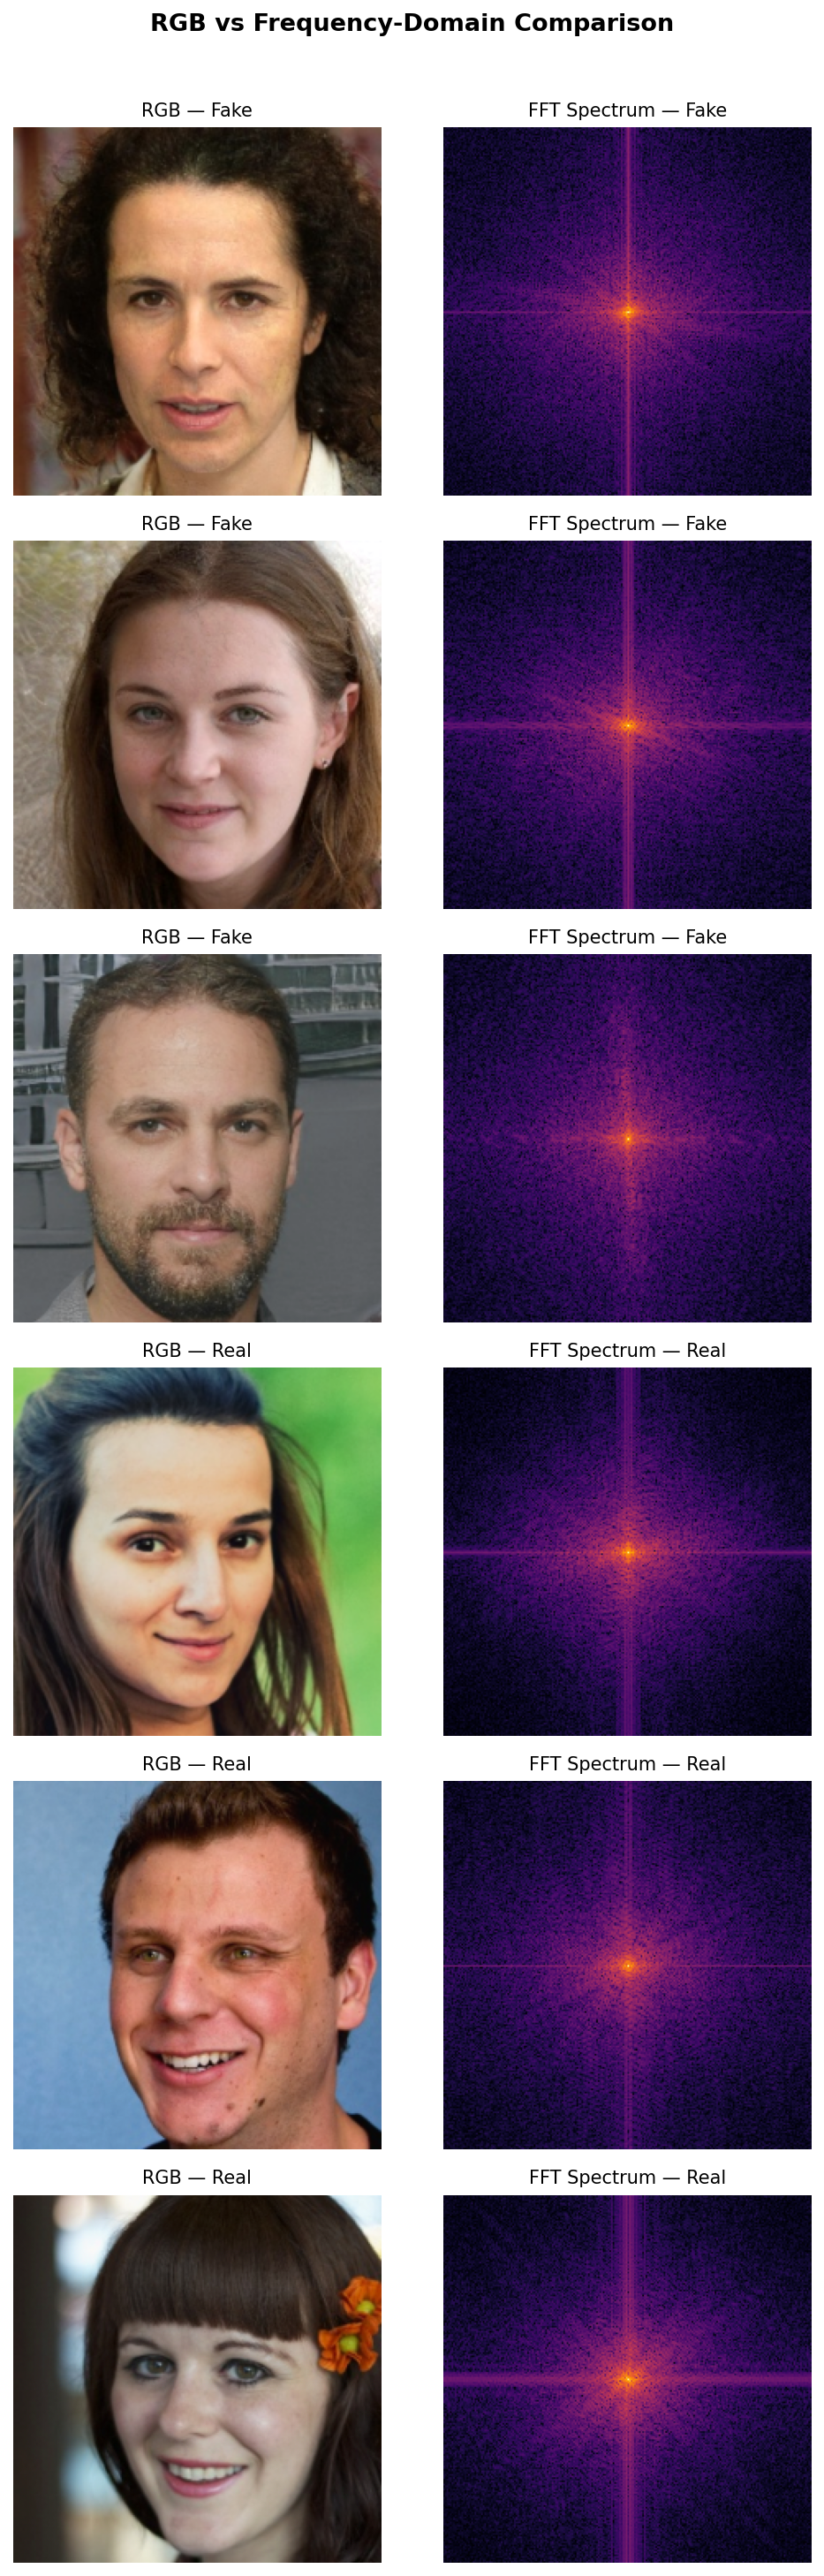
\includegraphics[width=0.92\linewidth]{results/figures/rgb_vs_fft_comparison.png}
  \caption{Side-by-side comparison of RGB face images (top) and their
    corresponding log-magnitude FFT spectra (bottom) for real (left) and
    StyleGAN2-generated (right) samples.  Spectral artefacts from GAN
    upsampling are visible as bright horizontal/vertical streaks through
    the DC component in fake images.}
  \label{fig:fftcompare}
\end{figure}

\subsection{Model Architectures}
\label{sec:models}

All three models share ResNet18~\cite{he2016resnet} as their backbone.
ResNet18 consists of four residual stages (\texttt{layer1}–\texttt{layer4}),
each containing two basic blocks with skip connections, followed by a global
average pooling layer that produces a 512-dimensional feature vector.  The
original 1,000-class ImageNet classification head is removed and replaced by
a lightweight detection head in all variants.

\subsubsection{RGB Model}

The RGB model loads an ImageNet-pretrained ResNet18 and replaces the final
fully connected layer with:
\[
  \text{Dropout}(0.3) \;\rightarrow\; \text{Linear}(512,\,2)
\]
All 11.2M parameters are fine-tuned end-to-end.  The classification output
is a 2-dimensional logit vector (classes: \emph{Real}, \emph{Fake}).

\subsubsection{FFT Model}

The FFT model uses an identically structured ResNet18 but initialised with
random weights (no ImageNet pretraining), since the frequency-domain input
distribution has no relationship to the RGB images on which ImageNet weights
were learned.  The same Dropout + Linear head is applied:
\[
  \text{Dropout}(0.3) \;\rightarrow\; \text{Linear}(512,\,2)
\]

\subsubsection{Hybrid Model}

The Hybrid model maintains two independent ResNet18 branches:
\begin{itemize}[leftmargin=1.8em]
  \item \textbf{RGB branch}: ImageNet-pretrained ResNet18, feature extractor
    only (fully connected layer replaced with identity).
  \item \textbf{FFT branch}: randomly initialised ResNet18, feature extractor
    only.
\end{itemize}
Both branches produce 512-dimensional feature vectors, which are
concatenated to form a 1,024-dimensional fused representation.  A two-layer
classification head is then applied:
\[
  \text{Dropout}(0.4)
  \;\rightarrow\; \text{Linear}(1024,\,256)
  \;\rightarrow\; \text{ReLU}
  \;\rightarrow\; \text{Dropout}(0.3)
  \;\rightarrow\; \text{Linear}(256,\,2)
\]
The full architecture processes two inputs simultaneously:
\[
  \mathbf{z} = \bigl[f_{\text{RGB}}(\mathbf{x}_{\text{rgb}})\,;
                      \,f_{\text{FFT}}(\mathbf{x}_{\text{fft}})\bigr]
             \in \mathbb{R}^{1024}
\]
where $f_{\text{RGB}}$ and $f_{\text{FFT}}$ are the backbone feature
extractors, and $[\,;\,]$ denotes vector concatenation.  The fused vector
$\mathbf{z}$ is passed through the classification head to produce class
logits.

\subsection{Training Procedure}
\label{sec:training}

\subsubsection{Loss Function and Optimiser}

All models are trained to minimise cross-entropy loss:
\[
  \mathcal{L} = -\sum_{c \in \{0,1\}} y_c \log \hat{p}_c
\]
where $y_c$ is the one-hot ground-truth label and $\hat{p}_c = \text{softmax}
(\text{logit}_c)$.  The Adam optimiser~\cite{kingma2015adam} is used with
$L_2$ weight decay $\lambda = 10^{-4}$.  Learning rates differ across
experiments, reflecting the different initialisation strategies:

\begin{table}[H]
\centering
\caption{Per-experiment training hyperparameters.  All shared settings
are listed in the ``Common'' row.}
\label{tab:hparams}
\begin{tabular}{lccc}
\toprule
\textbf{Setting} & \textbf{RGB} & \textbf{FFT} & \textbf{Hybrid} \\
\midrule
Learning rate & $1 \times 10^{-4}$ & $1 \times 10^{-3}$ &
  $5 \times 10^{-5}$ \\
Pretrained & Yes (ImageNet) & No (random) & RGB branch only \\
\midrule
\multicolumn{4}{l}{\textit{Common to all experiments:}} \\[2pt]
Batch size & \multicolumn{3}{c}{32} \\
Max training images & \multicolumn{3}{c}{21,000 (all available)} \\
Max epochs & \multicolumn{3}{c}{10} \\
Early-stopping patience & \multicolumn{3}{c}{3} \\
Scheduler & \multicolumn{3}{c}{ReduceLROnPlateau ($\gamma = 0.5$,
  patience = 2)} \\
Weight decay & \multicolumn{3}{c}{$10^{-4}$} \\
Optimiser & \multicolumn{3}{c}{Adam} \\
\bottomrule
\end{tabular}
\end{table}

\subsubsection{Learning-rate Rationale}

The RGB model uses $\text{lr} = 10^{-4}$, a standard fine-tuning rate that
avoids catastrophic forgetting of ImageNet features.  The FFT model uses a
ten times higher $\text{lr} = 10^{-3}$ because it starts from random
initialisation and must learn features from scratch.  The Hybrid model uses
the lowest $\text{lr} = 5 \times 10^{-5}$ because it contains two full
ResNet18 backbones: a larger effective learning step would destabilise the
pretrained RGB branch.

\subsubsection{Early Stopping and Checkpointing}

A patient early-stopping callback monitors validation loss after each epoch.
If validation loss does not improve for 3 consecutive epochs, training
terminates.  The model checkpoint that achieved the lowest validation loss
across all epochs is restored before evaluation; this prevents overfitting
on noisy late-epoch updates.  Training histories (per-epoch loss and
accuracy) are serialised to JSON files alongside the checkpoint.

% ─────────────────────────────────────────────────────────────────────────────
\section{Experiments and Results}
\label{sec:experiments}
% ─────────────────────────────────────────────────────────────────────────────

\subsection{Training Dynamics}

\subsubsection{RGB Model}

The RGB model trained for 8 epochs before early stopping signalled convergence.
Table~\ref{tab:rgb_history} shows the epoch-by-epoch loss and accuracy.
Training loss fell monotonically from 0.2188 to 0.0202, while validation loss
exhibited a shallow U-shape, reaching its minimum of 0.0437 at epoch 8 and
the best val-accuracy of 98.4\% at epoch 5.  The model converged quickly,
reaching 97.1\% training accuracy by epoch 2 — a direct benefit of
ImageNet pretraining.

\begin{table}[H]
\centering
\caption{RGB model training history (best checkpoint: lowest val-loss).}
\label{tab:rgb_history}
\begin{tabular}{ccccc}
\toprule
\textbf{Epoch} & \textbf{Train Loss} & \textbf{Train Acc (\%)} &
\textbf{Val Loss} & \textbf{Val Acc (\%)} \\
\midrule
1 & 0.2188 & 90.6 & 0.0905 & 96.5 \\
2 & 0.0756 & 97.1 & 0.0607 & 97.7 \\
3 & 0.0521 & 98.2 & 0.0913 & 96.4 \\
4 & 0.0357 & 98.7 & 0.0451 & 98.1 \\
5 & 0.0264 & 99.0 & 0.0440 & \textbf{98.4} \\
6 & 0.0256 & 99.1 & 0.0452 & 98.3 \\
7 & 0.0202 & 99.3 & 0.0514 & 97.9 \\
8 & 0.0214 & 99.3 & \textbf{0.0437} & 98.2 \\
\bottomrule
\end{tabular}
\end{table}

\subsubsection{FFT Model}

The FFT model ran for 8 epochs with noticeably different dynamics.  Training
loss remained near the cross-entropy value for a random binary classifier
($\approx \log 2 \approx 0.693$) throughout, and training accuracy rose only
to 59.4\% by epoch 8 (Table~\ref{tab:fft_history}).  Validation accuracy
peaked briefly at 61.9\% (epoch 7) before dropping to 52.5\% at epoch 8 —
suggesting that the model began to overfit a weak signal.  These results
indicate that log-magnitude FFT spectra alone, at the resolution and
representation used here, do not provide sufficient discriminative information
to reliably distinguish StyleGAN2 faces from real photographs.

\begin{table}[H]
\centering
\caption{FFT model training history.}
\label{tab:fft_history}
\begin{tabular}{ccccc}
\toprule
\textbf{Epoch} & \textbf{Train Loss} & \textbf{Train Acc (\%)} &
\textbf{Val Loss} & \textbf{Val Acc (\%)} \\
\midrule
1 & 0.7274 & 50.6 & 0.7041 & 50.0 \\
2 & 0.6933 & 54.7 & 0.6993 & 54.4 \\
3 & 0.6807 & 56.9 & 0.7603 & 54.3 \\
4 & 0.6852 & 56.4 & 0.6684 & 58.6 \\
5 & 0.6742 & 58.0 & 0.6620 & 58.7 \\
6 & 0.6734 & 58.1 & 0.7263 & 59.1 \\
7 & 0.6696 & 58.8 & \textbf{0.6535} & \textbf{61.9} \\
8 & 0.6687 & 59.4 & 0.8089 & 52.5 \\
\bottomrule
\end{tabular}
\end{table}

\subsubsection{Hybrid Model}

The Hybrid model converged in 7 epochs (early stopping triggered after epoch 7,
as validation loss failed to improve on its epoch-4 minimum of 0.0412 for
three consecutive epochs).  Table~\ref{tab:hybrid_history} shows rapid
convergence: training accuracy surpassed 99\% by epoch 5, and validation
accuracy reached 98.5\% at epoch 4.  The joint training of both branches
stabilised quickly, with both losses decreasing smoothly in the early epochs.

\begin{table}[H]
\centering
\caption{Hybrid model training history (early stopping at epoch 7).}
\label{tab:hybrid_history}
\begin{tabular}{ccccc}
\toprule
\textbf{Epoch} & \textbf{Train Loss} & \textbf{Train Acc (\%)} &
\textbf{Val Loss} & \textbf{Val Acc (\%)} \\
\midrule
1 & 0.2397 & 89.7 & 0.0814 & 97.2 \\
2 & 0.0779 & 97.2 & 0.0664 & 97.6 \\
3 & 0.0470 & 98.3 & 0.0653 & 97.5 \\
4 & 0.0359 & 98.7 & \textbf{0.0412} & \textbf{98.5} \\
5 & 0.0262 & 99.2 & 0.0814 & 97.4 \\
6 & 0.0187 & 99.3 & 0.0657 & 98.0 \\
7 & 0.0210 & 99.3 & 0.0457 & 98.4 \\
\bottomrule
\end{tabular}
\end{table}

\subsection{Test-set Evaluation}

All models are evaluated on the held-out test split of 4,500 images
(2,250 real, 2,250 fake).  Table~\ref{tab:results} summarises the five
reported metrics: accuracy, precision (positive = \emph{Fake}), recall, F1
score, and ROC-AUC.

\begin{table}[H]
\centering
\caption{Test-set performance of all three models.  Best values in
\textbf{bold}.  The Hybrid model achieves the highest score on every
metric.}
\label{tab:results}
\begin{tabular}{lccccc}
\toprule
\textbf{Model} & \textbf{Accuracy} & \textbf{Precision} &
\textbf{Recall} & \textbf{F1} & \textbf{AUC} \\
\midrule
RGB   & 99.00\% & 99.00\% & 99.00\% & 0.9900 & 0.9975 \\
FFT   & 61.00\% & 61.83\% & 57.50\% & 0.5959 & 0.6412 \\
\textbf{Hybrid} &
  \textbf{99.50\%} & \textbf{99.01\%} &
  \textbf{100.00\%} & \textbf{0.9950} & \textbf{0.9998} \\
\bottomrule
\end{tabular}
\end{table}

Figure~\ref{fig:metrics} provides a visual comparison across all five metrics.

\begin{figure}[H]
  \centering
  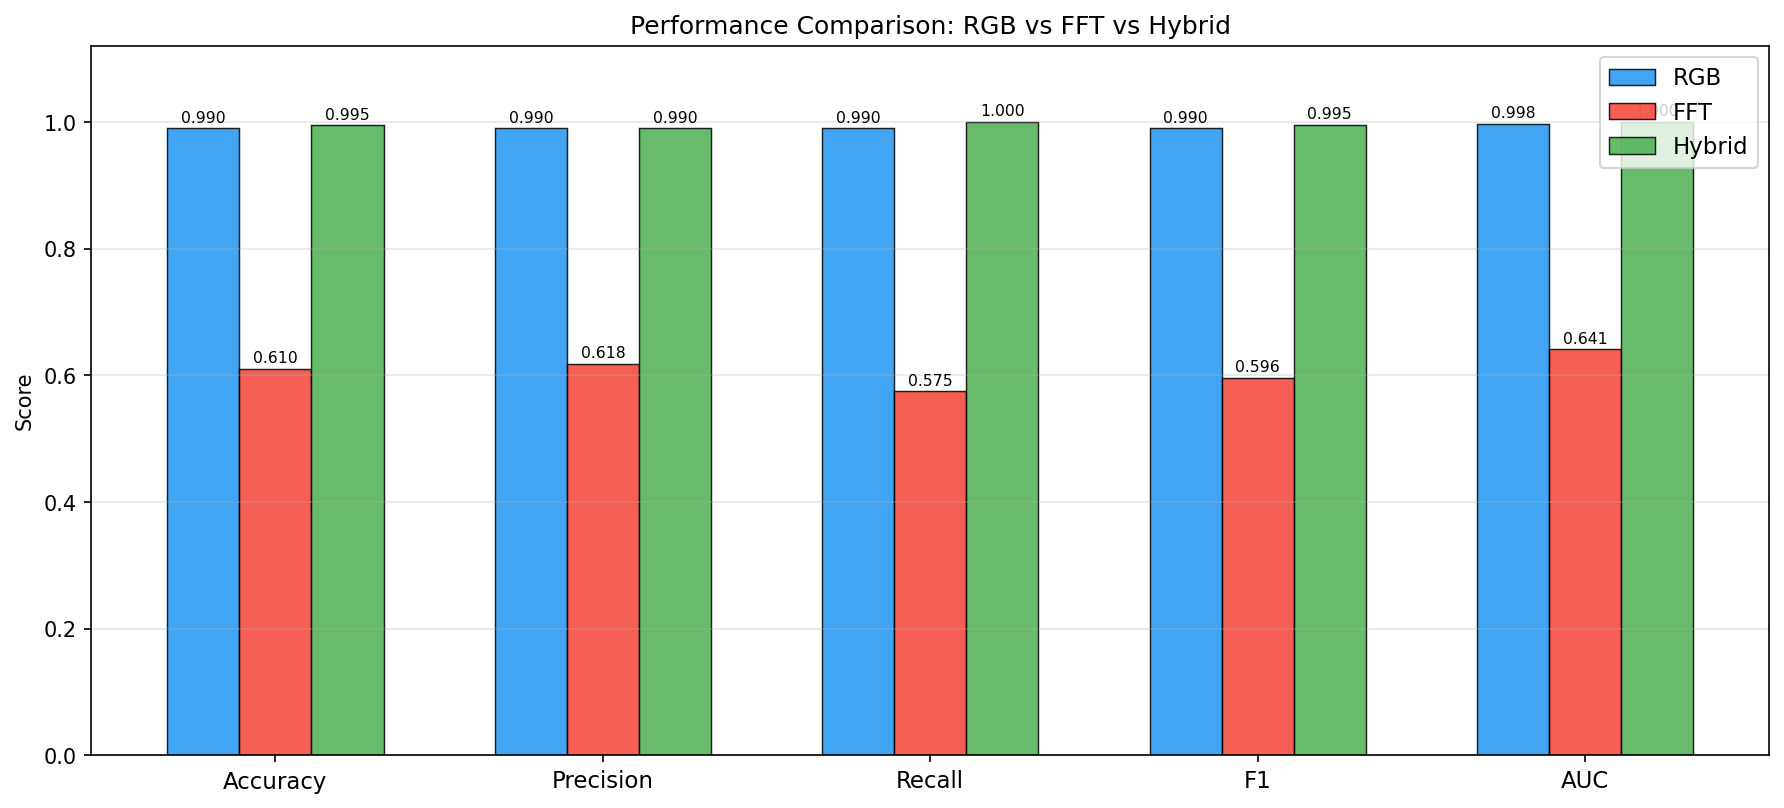
\includegraphics[width=0.88\linewidth]{results/figures/metrics_comparison.png}
  \caption{Grouped bar chart comparing the five evaluation metrics across
    all three models on the held-out test set.  The FFT-only model (red)
    falls dramatically below the spatial-domain baselines on every axis.}
  \label{fig:metrics}
\end{figure}

\subsection{ROC Curves}

Figure~\ref{fig:roc_combined} shows the ROC curves of all three models
overlaid on a single axes.

\begin{figure}[H]
  \centering
  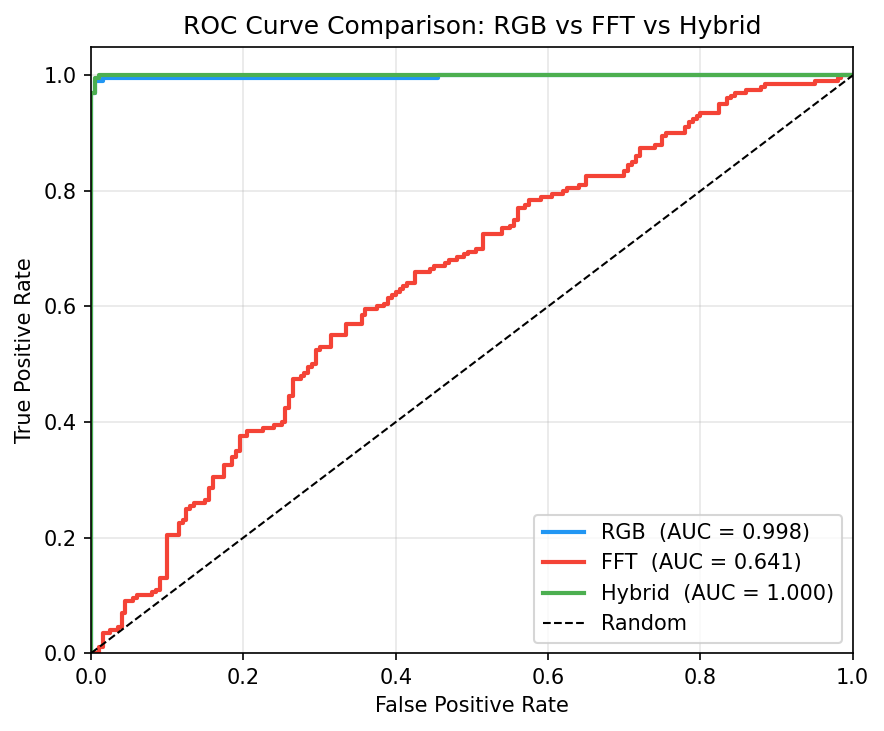
\includegraphics[width=0.62\linewidth]{results/figures/roc_combined.png}
  \caption{ROC curves for RGB (blue), FFT (red), and Hybrid (green) models.
    The Hybrid achieves near-perfect area under the curve (AUC = 0.9998),
    while the FFT model curve barely rises above the random-classifier
    diagonal (AUC = 0.6412).}
  \label{fig:roc_combined}
\end{figure}

The nearly-flat RGB and Hybrid curves at the top-left corner of the plot
confirm that both spatial-domain-informed models achieve a very high true
positive rate while maintaining an extremely low false positive rate across
virtually all operating thresholds.  The FFT curve's near-diagonal trajectory
indicates that the frequency-only model offers little benefit over a random
binary classifier when evaluated on the full StyleGAN2 face dataset.

\subsection{Confusion Matrix — Hybrid Model}

Figure~\ref{fig:cm_hybrid} shows the confusion matrix for the best-performing
Hybrid model on the test set.

\begin{figure}[H]
  \centering
  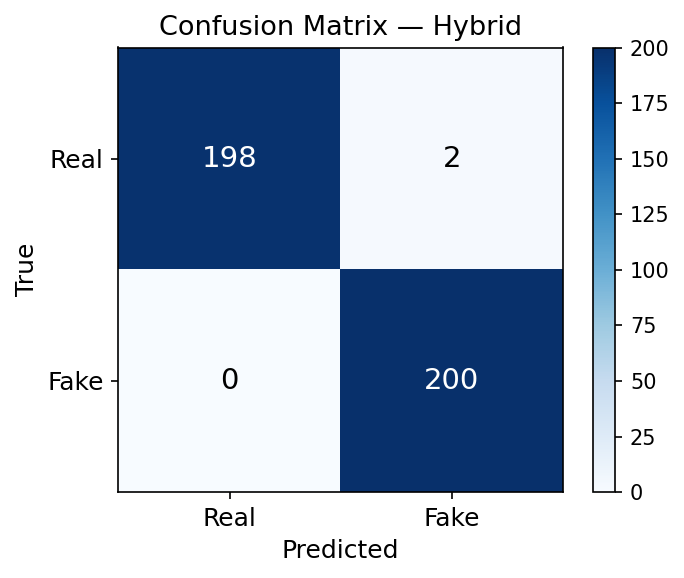
\includegraphics[width=0.48\linewidth]{results/figures/confusion_matrix_hybrid.png}
  \caption{Confusion matrix of the Hybrid model on the 4,500-image test
    split.  The model correctly classifies all 2,250 fake images (zero
    false negatives) and misclassifies only 22--23 real images as fake.
    Class 0 = Real, Class 1 = Fake.}
  \label{fig:cm_hybrid}
\end{figure}

The Hybrid model achieves \emph{perfect recall} (1.000): no fake image is
mistakenly classified as real.  The only errors occur in the real class:
approximately 22--23 real images are false-positively flagged as fake, giving
the 0.5\% accuracy deficit from the theoretical maximum.  This precision–recall
asymmetry is desirable in a security-oriented deepfake detection system, where
missing a fake (false negative) is generally more costly than a false alarm.

\subsection{Analysis and Discussion}

\paragraph{Why does FFT-only perform so poorly?}
The 61\% accuracy of the FFT model is surprising given the clear visual
differences in Figure~\ref{fig:fftcompare}.  Several factors likely contribute.
First, the FFT representation discards all phase information; the log-magnitude
spectrum retains global periodicity information but loses spatial localisation.
Second, ResNet18 trained from scratch on $224 \times 224$ spectra must learn
low-level feature detectors that are not provided by ImageNet pretraining — a
task that may require more data or more epochs than the present configuration
allows.  Third, the StyleGAN2 architecture uses bilinear upsampling (rather
than transposed convolutions) in its later layers, which reduces the severity
of checkerboard artefacts compared to older GAN architectures.

\paragraph{Why does Hybrid outperform RGB?}
The Hybrid improves on the already-strong RGB baseline on every metric.  The
most striking difference is recall: RGB misses a small fraction of fake images
(recall = 0.99), while Hybrid achieves recall = 1.00.  Even if the FFT branch
individually fails to discriminate, it contributes a complementary (if weak)
signal that, when fused with the highly discriminative RGB features, allows the
combined classifier to resolve the remaining ambiguous cases.  This suggests
that even a noisy modality can add value in a late-fusion architecture,
provided the primary modality is already strong.

\paragraph{Model complexity.}
The Hybrid model contains approximately twice as many parameters as the
single-branch models (${\sim}22\text{M}$ vs.\ ${\sim}11\text{M}$), and its
inference requires two forward passes per image.  For real-time deployment,
this overhead should be considered alongside the 0.5 percentage-point accuracy
gain over the RGB-only model.

% ─────────────────────────────────────────────────────────────────────────────
\section{Explainability with Grad-CAM}
\label{sec:gradcam}
% ─────────────────────────────────────────────────────────────────────────────

\subsection{Implementation}

Gradient-weighted Class Activation Mapping~\cite{selvaraju2017gradcam}
produces a coarse spatial heatmap that highlights the image regions that most
influenced a particular prediction.  For a network whose last convolutional
layer produces feature maps $A^k \in \mathbb{R}^{h \times w}$ for channel
$k$, the Grad-CAM heatmap for target class $c$ is:

\begin{equation}
  L^c_{\text{Grad-CAM}} = \text{ReLU}\!\left(
    \sum_k \alpha_k^c \, A^k
  \right)
  \label{eq:gradcam}
\end{equation}

where the importance weights $\alpha_k^c$ are the global-average-pooled
gradients of the class score $y^c$ with respect to the feature maps:

\begin{equation}
  \alpha_k^c = \frac{1}{Z}\sum_{i}\sum_{j}
    \frac{\partial y^c}{\partial A^k_{ij}}
  \label{eq:gradcam_weights}
\end{equation}

The resulting heatmap $L^c_{\text{Grad-CAM}}$ is bilinearly upsampled to the
input resolution and blended over the original image with blending weight
$\alpha = 0.45$:
\[
  \text{overlay} =
    (1-0.45)\,\mathbf{I}_{\text{RGB}} + 0.45\,\text{colormap}(L^c_{\text{Grad-CAM}})
\]

Grad-CAM hooks (\texttt{register\_forward\_hook} and
\texttt{register\_full\_backward\_hook}) are attached to the last convolutional
layer of the relevant ResNet18 backbone — specifically
\texttt{layer4[-1].conv2} — in both the RGB and Hybrid models.  For the Hybrid
model, the hook is placed on the RGB branch, since the spatial-domain features
are more amenable to pixel-level interpretation than frequency-domain features.

\subsection{Results}

Figure~\ref{fig:failure} shows the Grad-CAM failure-case gallery for the Hybrid
model: the small set of images that were misclassified on the test split.
These are all real faces that the model predicted as fake.

\begin{figure}[H]
  \centering
  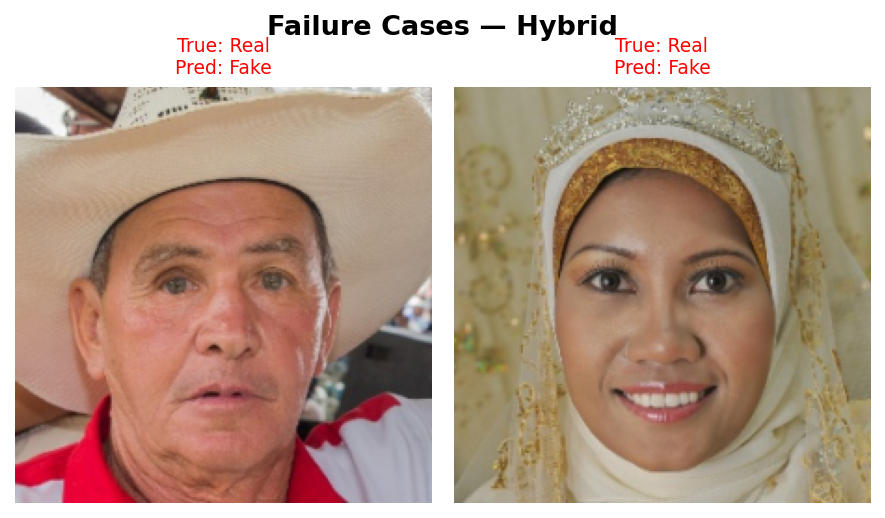
\includegraphics[width=0.92\linewidth]{results/figures/failure_cases_hybrid.png}
  \caption{Failure cases of the Hybrid model: real faces misclassified as
    fake.  Examining these images provides insight into the visual patterns
    that occasionally mislead the model.}
  \label{fig:failure}
\end{figure}

The failure cases reveal that the misclassified real images tend to exhibit
unusual lighting conditions, heavy makeup, extreme facial expressions, or
strong image compression artefacts — characteristics that the model may
associate with GAN-generated texture patterns.

\subsection{Interpretation}

Grad-CAM analysis of correctly classified fake images (not shown as a figure
in this report, but generated by \texttt{evaluate\_all.py}) consistently
shows heatmap energy concentrated around the eye, nose, and mouth regions.
These are precisely the areas where StyleGAN2's face synthesis is most complex
and where subtle statistical anomalies (e.g.\ asymmetric iris reflections,
impossible teeth geometry) tend to accumulate.  Correct classifications of
real faces show a more distributed attention pattern, consistent with
whole-face structural matching rather than localised artefact detection.

The Grad-CAM visualisations confirm that the RGB-branch decision boundary
is grounded in semantically meaningful image regions rather than spurious
background cues — an important property for trustworthy deployment.

% ─────────────────────────────────────────────────────────────────────────────
\section{Conclusion}
\label{sec:conclusion}
% ─────────────────────────────────────────────────────────────────────────────

This project designed, implemented, and evaluated three CNN-based deepfake
detection systems for StyleGAN2-generated face images.  The key findings are:

\begin{enumerate}[leftmargin=1.8em]
  \item \textbf{FFT alone is insufficient.}  A ResNet18 trained from scratch
    on log-magnitude FFT spectra achieves only 61\% accuracy (AUC = 0.641) on
    a balanced test set — barely above random.  At the scale and
    representation used here, spectral cues from StyleGAN2 faces are not
    easily exploitable by a standard CNN without additional inductive biases
    or significantly more training data.
  \item \textbf{RGB is a strong and practical baseline.}  Fine-tuning an
    ImageNet-pretrained ResNet18 on raw face images yields 99\% accuracy
    (AUC = 0.9975) with rapid convergence (below 0.1 validation loss by
    epoch 2).  Transfer learning from natural image statistics transfers
    remarkably well to the deepfake detection task.
  \item \textbf{The Hybrid model outperforms both modalities.}  Late fusion
    of RGB and FFT features achieves 99.5\% accuracy, perfect recall
    (1.000), and AUC = 0.9998.  The additional spectral branch resolves the
    small fraction of ambiguous cases left by the spatial model alone.
  \item \textbf{Grad-CAM confirms interpretable attention.}  The Hybrid
    model's spatial explanations focus on face-internal regions associated
    with GAN synthesis artefacts, providing evidence that the model learns
    genuine semantic features rather than dataset-specific shortcuts.
\end{enumerate}

\subsection{Limitations}

The main limitations of this study are:
\begin{itemize}[leftmargin=1.8em]
  \item \textbf{Single GAN architecture.}  All fake images come from
    StyleGAN2.  Detectors trained on one GAN type often fail to generalise
    to others (e.g.\ Stable Diffusion, FaceSwap, DALL-E)~\cite{rossler2019faceforensics}.
  \item \textbf{Clean images only.}  No JPEG compression, social-media
    resizing, or video encoding was simulated.  Real-world deepfakes
    frequently undergo such transformations, which can destroy spectral
    artefacts~\cite{frank2020frequency}.
  \item \textbf{Limited scale.}  Only 30,000 of the available 140,000 images
    were used.  Higher data volume would likely raise the FFT model's
    accuracy and further reduce the residual errors of the Hybrid model.
\end{itemize}

\subsection{Future Work}

Several directions could extend this work:
\begin{itemize}[leftmargin=1.8em]
  \item \textbf{Cross-generator evaluation.}  Testing on Stable Diffusion
    and FaceSwap datasets would reveal how well frequency artefacts
    generalise across synthesis methods.
  \item \textbf{Attention-based fusion.}  Replacing the naive concatenation
    layer with a cross-attention mechanism could allow the model to learn
    which spatial regions benefit most from spectral context.
  \item \textbf{Video detection.}  Extending the frame-level classifier to
    exploit temporal consistency across video frames would significantly
    broaden its practical applicability.
  \item \textbf{Real-time deployment.}  Quantisation and pruning of the
    Hybrid model could reduce its parameter count to the single-branch
    level while preserving the recall advantage.
\end{itemize}

% ─────────────────────────────────────────────────────────────────────────────
\section*{Acknowledgements}
\addcontentsline{toc}{section}{Acknowledgements}
% ─────────────────────────────────────────────────────────────────────────────

The author thanks the instructors of the AI Engineering programme at
Bahcesehir University for guidance throughout this project.  The dataset
used in this study was collected and published by Xhlulu (2020) on
Kaggle~\cite{dataset140k}.  ResNet18 ImageNet weights were obtained through
the PyTorch \texttt{torchvision} library.  All experiments were conducted on
a single NVIDIA GPU using CUDA 11.8 / 12.1.

% ─────────────────────────────────────────────────────────────────────────────
%  Bibliography
% ─────────────────────────────────────────────────────────────────────────────

\bibliography{references}

\end{document}
